\chapter{Validación de la solución}\label{chap:3}

En este capítulo se se valida el correcto funcionamiento de la funcionalidad implementada. Además, a partir de los datos importados y transformados, se demuestra que es posible formar equipos en ambos contextos utilizando la herramienta TEAMSOFT$^+$.

\section{Importación de los datos de los docentes}\label{sec:impo_docencia}
A continuación se describe el proceso de importación para el caso específico del problema de la docencia. Para iniciar este proceso se seleccionó el fichero que se muestra en el Anexo \ref{fig:fichero-docencia}. La Tabla \ref{table:importar-fichero-docencia} describe brevemente su contenido.\\

En este ejemplo el fichero contiene 16 profesores pertenecientes a la disciplina docente: Inteligencia Computacional de la Facultad de Ingeniería Informática. Estos profesores se insertan en un nuevo grupo: \textbf{profesores IC}. En el Anexo \ref{fig:cargar-fichero-docencia} se presenta el resultado de este paso. A continuación se mapean los atributos del fichero y las características de las personas. En el ejemplo se seleccionan los atributos del fichero: \textbf{nombre}, \textbf{exp} y se asocian con las características de las personas: \textbf{Nombre} y \textbf{Experiencia} (ver Anexo \ref{fig:mapeo_atr_pers}). En la Tabla \ref{table:mapeo_competencias_docencia} se ejemplifica la variante utilizada para realizar el mapeo de los atributos del fichero con las competencias. A partir de este mapeo es necesario definir el peso correspondiente a cada una de las categorías establecidas para las competencias. 

\begin{table}[H]
	\centering
	\caption{Descripción de los atributos que se manejan en el fichero docencia}\label{table:importar-fichero-docencia}
	\scalebox{.9}{
	\begin{tabular} {l | p{10cm}}
		\toprule
		\textbf{Atributo} & \textbf{Descripción} \\ \midrule
		nombre & Nombre de los profesores \\ \hline
		exp & Años de experiencia laboral de los profesores \\ \hline
		cd & Categoría docente \\ \hline
		cc & Categoría científica \\ \hline
		trabdoc & Evaluación del profesor en el trabajo docente \\ \hline
		trabmet & Evaluación del profesor en el trabajo metodológico\\ \hline
		trabinv & Evaluación del profesor en el trabajo investigativo\\ \hline
		conf & Experiencia del profesor trabajando en el rol de conferencia\\ \hline
		cpractica & Experiencia del profesor trabajando en el rol de clase práctica \\ \hline
		seminario & Experiencia del profesor trabajando en el rol de seminario\\ \hline\\
		lab & Experiencia del profesor trabajando en el rol de Laboratorio\\ \hline\\
		tall & Experiencia del profesor trabajando en el rol de taller \\ \hline\\
		jefeasig & Experiencia del profesor trabajando en el rol de Líder\\ \bottomrule
	\end{tabular}
}
\end{table}

\begin{table}[H]
	\centering
	\caption{Mapeo atributos del fichero con las competencias}\label{table:mapeo_competencias_docencia}
%	\scalebox{.9}{
	\begin{tabular} {l | l}
		\toprule
		\textbf{Atributo fichero} & \textbf{Competencia} \\ \midrule
		cd & Categoría Docente \\ \hline
		cc & Grado científico \\ \hline
		trabdoc & Trabajo docente \\ \hline
		trabmet & Trabajo metodológico \\ \hline
		trabinv & Trabajo investigativo \\ \bottomrule
	\end{tabular}
%}
\end{table}

En este caso, el formato de los atributos asociados es de tipo texto, por lo que hay que se asignar directamente el valor del peso de cada uno de ellos, teniendo que cumplir la condición de que la suma de todos ellos sea igual a uno. En la Tabla \ref{table:config_competencias_docencia} se muestra la asignación de los pesos para el atributo \textbf{cd}; las configuraciones para el resto de los atributos se pueden consultar en los Anexos \ref{fig:conf_comp_cc_docencia}, \ref{fig:conf_comp_doc_docencia} y \ref{fig:conf_comp_inv_docencia}. Para asociar los atributos del fichero a los roles, se siguieron las configuraciones establecidas en la Tabla \ref{table:mapeo_roles_docencia}.

{\hspace{-1.2cm}
\begin{tabular}{cc}
	
    \begin{minipage}{8cm}
      \begin{table}[H]
    	\centering
    	
    	\caption{Configuración del atributo cd}\label{table:config_competencias_docencia}
		\scalebox{.9}{
      	\begin{tabular} {l | l}
	    	\toprule
	    	\textbf{Valor del atributo} & \textbf{Peso} \\ \midrule
			Titular & 0.4 \\ \hline
			Auxiliar & 0.3 \\ \hline
			Instructor & 0.1 \\ \hline
			Asistente & 0.15 \\ \hline
			Instructor recién graduado & 0.05  \\ \hline		
			\textbf{Suma} & \textbf{1} \\ \bottomrule
		\end{tabular}
	}
	\end{table}

	\end{minipage}
&
	\begin{minipage}{8cm}

		\begin{table}[H]
			\centering
			\caption{Mapeo de atributos con los roles}\label{table:mapeo_roles_docencia}
		\scalebox{.9}{
			\begin{tabular} {l | l}
				\toprule
				\textbf{Valor del atributo} & \textbf{Rol} \\ \midrule
				jefeasig & Líder \\ \hline
				tall & Taller \\ \hline
				lab & Laboratorio \\ \hline
				sem & Seminario \\ \hline
				cpractica & Clase Práctica  \\ \hline		
				conf & Conferencia \\ \bottomrule
			\end{tabular}
	}
		\end{table}
	\end{minipage}
\end{tabular}}\\

El sistema permite que las configuraciones anteriores puedan se editadas en el último paso justo antes de realizar la importación de las personas (ver Anexo \ref{fig:verificar_datos_docencia}). Al finalizar el proceso, se muestra un mensaje informando al usuario el resultado de la importación (ver Anexo \ref{fig:resultados_docencia}). El resultado final de la importación se puede consultar en el Anexo \ref{fig:lista_profesores_docencia}. Los datos de un profesor en particular, en este caso el profesor Milton, pueden ser consultados en los Anexos \ref{fig:comp_genericas_docencia}, \ref{fig:comp_tecnicas_docencia}, \ref{fig:pref_roles_docencia}.

\section{Importación de los datos de  béisbol} \label{sec:impo_beisbol}
A continuación se describe el proceso de importación para el caso específico del problema del béisbol. Para iniciar este proceso se seleccionó el fichero que se muestra en el Anexo \ref{fig:fichero-beisbol}. Este fichero almacena los atributos obligatorios de las personas como son la experiencia y el nombre de cada uno. En adición se almacenan las estadísticas de las personas para los indicadores definidos en la Tabla \ref{correspondencia-pel}, así como los años de experiencia en cada rol.\\

En este ejemplo el fichero contiene 24 jugadores pertenecientes al equipo de la Serie Nacional de Matanzas. Estos jugadores se insertan en un nuevo grupo: \textbf{staff matanzas}. En el Anexo \ref{fig:cargar-fichero-docencia} se presenta el resultado de este paso. A continuación se mapean los atributos del fichero y las características de los jugadores. En el ejemplo se seleccionan los atributos del fichero: \textbf{nombre}, \textbf{exp} y se asocian con las características de las personas: \textbf{Nombre} y \textbf{Experiencia} (ver Anexo \ref{fig:mapeo_atr_pers}). En la Tabla \ref{table:mapeo_competencias_beisbol} se ejemplifica la variante utilizada para realizar el mapeo de los atributos del fichero con las competencias. A partir de este mapeo se logra definir a partir de qué atributos se van a calcular las competencias.

\begin{table}[H]
	\centering
	\caption{Mapeo de atributos del fichero con las competencias}\label{table:mapeo_competencias_beisbol}
	\scalebox{.9}{
		\begin{tabular} {l | p{9cm}}
			\toprule
			\textbf{Atributo fichero} & \textbf{Competencia} \\ \midrule
			ci & batear con hombres en base \\ \hline
			 sh&   batear con hombres en base, capacidad de embase \\ \hline
			sf &  batear con hombres en base \\ \hline
			cipa &   batear con hombres en base\\ \hline
			dobles &  fuerza de bateo, velocidad \\ \hline
			triples & fuerza de bateo, velocidad  \\ \hline
			hr &   fuerza de bateo\\ \hline
			slu &   fuerza de bateo\\ \hline
			obp & capacidad de embase  \\ \hline
			avgO & capacidad de embase   \\ \hline
			avgD & precisión de tiro \\ \hline
			br &  velocidad, capacidad de embase \\ \hline
			cr &   velocidad \\ \bottomrule
		\end{tabular}
	}
\end{table}

En este caso, existen más de un atributo que tiene relación con una competencia, por lo que hay que asignar directamente el valor del peso de cada uno de ellos, teniendo que cumplir la condición de que la suma de todos ellos sea igual a uno. En la Tabla \ref{table:config_competencias} se muestra la asignación de los pesos para la competencia \textbf{batear con hombres en base}; las configuraciones para el resto de las competencias se pueden consultar en los Anexos \ref{fig:conf_comp_ce_beisbol}, \ref{fig:conf_comp_fb_beisbol} y \ref{fig:conf_comp_v_beisbol}. Además, todos los atributos seleccionados que tienen relación con las competencias son de tipo numérico. Por lo que hay que definir el máximo valor a tener en cuenta para cada uno de ellos. Por defecto, el sistema busca en el fichero de entrada, el máximo valor para cada atributo.

\begin{table}[H]
	\centering
	\caption{Configuración de la competencia  \textbf{batear con hombres en base}}\label{table:config_competencias}
	\scalebox{.9}{
		\begin{tabular} {l | l}
			\toprule
			\textbf{Atributo} & \textbf{Peso} \\ \midrule
				ci & 0.4 \\ \hline
				sh & 0.2 \\ \hline
				sf & 0.1 \\ \hline
				cipa & 0.3 \\ \hline
			\textbf{Suma} & \textbf{1} \\ \bottomrule
		\end{tabular}
	}
\end{table}

Para asociar los atributos del fichero a los roles, se siguieron las configuraciones establecidas en la Tabla \ref{mapeo-tipo-roles}. Como casos especiales (porque no son roles ofensivos o defensivos), los atributos \textit{banco} y \textit{capitan} se mapean con sus correspondientes \textit{Banco} y \textit{Líder}.

\begin{table}[H]
	\centering
	\caption{Mapeo de los atributos por tipo de rol}\label{mapeo-tipo-roles}
%	\scalebox{0.95}{
		\begin{tabular}{c l c l}
			\toprule
			\textbf{Atributo} & \textbf{Roles defensivos} & \textbf{Atributo} & \textbf{Roles Ofensivos} \\ \midrule
			C                 & catcher                   & B1                & primer bate              \\
			1B          & primera base              & B2                & segundo bate             \\
			2B          & segunda base              & B3                & tercer bate              \\
			SS                & campo corto               & B4                & cuarto bate              \\
			3B          & tercera base              & B5                & quinto bate              \\
			LF                & jardinero izquierdo       & B6                & sexto bate               \\
			CF                & jardinero central         & B7                & séptimo bate             \\
			RF                & jardinero derecho         & B8                & octavo bate              \\
			BD                & bateador designado        & B9                & noveno bate              \\ \bottomrule
		\end{tabular}
%	}
\end{table}


El sistema permite que las configuraciones anteriores puedan se editadas en el último paso justo antes de realizar la importación de las personas (ver Anexo \ref{fig:verificar_datos_beisbol}). Al finalizar el proceso, se muestra un mensaje informando al usuario el resultado de la importación (ver Anexo \ref{fig:resultados_beisbol}). El resultado final de la importación se puede consultar en el Anexo \ref{fig:lista_jugadores_beisbol}. Los datos de un jugador en particular, en este caso el jugador Santoya, pueden ser consultados en los Anexos \ref{fig:comp_genericas_beisbol}, \ref{fig:comp_tecnicas_beisbol}, \ref{fig:pref_roles_beisbol}.

\section{Limitaciones de la herramienta TEAMSOFT$^+$ para la solución de los problemas de formación de equipos de béisbol y docentes} \label{sec:limitaciones}

Es necesario comprobar que la herramienta TEAMSOFT$^+$ permite la formación de los equipos de béisbol y docentes siguiendo las adaptaciones propuestas para ambos problemas. En esta sección se le realizan algunas pruebas a la herramienta para comprobar su funcionamiento ante ambos problemas. Para llevar a cabo los Casos de Pruebas (CP) se vaciaron las tablas (de la base de datos) correspondientes a las competencias y roles. Esto persigue como objetivo simular la creación desde cero en ambos problemas. Como se observa en la Tabla \ref{t:casos-de-prueba-humo}, en los primeros cuatro CP se cumple lo esperado. Mientras que en el CP5, al momento que se intenta crear una nueva estructura, se presenta un error.

\begin{table}[H]
	\centering
	\caption{Prueba de humo crear equipo sin rol Jefe de equipo}\label{t:casos-de-prueba-humo}
	\scalebox{.75}{
		\begin{tabular}{c p{2.3cm} e{4.7cm} e{5cm} p{3cm} p{3cm}}
			\toprule
			\textbf{ID} & \textbf{Escenario}                                               & \item[]\textbf{Pasos}                                                                                                                                       & \item[]\textbf{Información de entrada}                                    & \textbf{Resultado esperado}               & \textbf{Resultado actual}                                                                                     \\ \midrule
			CP1     & Introducir roles sin que el nombre de ninguno sea Jefe de equipo & \item Introducir nombre
			\item Introducir descripción
			\item Establecer impacto
			\item Establecer competencias
			\item Establecer incompatibilidades & \item Primera Base 
			\item Jugador de cuadro
			\item 0.0
			\item Trabajo bajo presión (nivel: en partida, importancia: alguna medida)
			\item Ninguna
			& El rol debe insertarse sin problemas      & Se cumple lo esperado                                                                                         \\ \hline
			CP2     & Introducir roles sin que el nombre de ninguno sea Jefe de equipo & \item Introducir nombre
			\item Introducir descripción
			\item Establecer impacto
			\item Establecer competencias
			\item Establecer incompatibilidades & \item Segunda Base                                             
			\item Jugador de cuadro
			\item 0.0
			\item Trabajo bajo presión (nivel: en partida, importancia: alguna medida)
			\item Ninguna
			& El rol debe insertarse sin problemas      & Se cumple lo esperado                                                                                         \\ \hline
			CP3     & Introducir roles sin que el nombre de ninguno sea Jefe de equipo & \item Introducir nombre
			\item Introducir descripción
			\item Establecer impacto
			\item Establecer competencias
			\item Establecer incompatibilidades & \item Capitán       
			\item Líder del equipo
			\item 0.0
			\item Trabajo bajo presión (nivel: en partida, importancia: alguna medida)
			\item Ninguna
			& El rol debe insertarse sin problemas      & Se cumple lo esperado                                                                                         \\ \hline
			CP4     & Crear Proyecto                                                   & \item Abrir menú problema
			\item Introducir nombre
			\item Establecer fecha
			\item Seleccionar entidad
			\item Seleccionar provincia                  & \item Nuevo Problema 
			\item 12/10/2021
			\item Inder
			\item La Habana
			& Debe continuar con el proceso de creación & Se cumple lo esperado                                                                                         \\ \hline
			CP5     & Crear estructura del proyecto                                    & \item Introducir nombre nuevo
			\item Seleccionar roles
			\item Establecer cantidad de trabajadores
			\item \textit{Click} en: Siguiente                 & \item Nueva estructura
			\item Primera base, Segunda Base, Capitán
			\item uno por cada rol                                         
			
			& Mostrar mensaje creación de la estructura & Se muestra mensaje de error, informando que no hay un \textbf{Jefe de Proyecto} entre los roles seleccionados \\ \bottomrule
		\end{tabular}
	}
\end{table}

Reproduciendo los dos primeros CP de la Tabla \ref{t:casos-de-prueba-humo}, se lleva a cabo los mostrados en la Tabla \ref{t:casos-de-prueba-humo2}. En este caso queda claro que resulta necesario para crear una nueva estructura, la existencia de un rol con el nombre \textit{Jefe de Proyecto} (ver Figura \ref{fig:error-jefe-proy}).


\begin{table}[H]
	
%	\centering
	\caption{Prueba de humo crear proyecto con rol Jefe de Proyecto}\label{t:casos-de-prueba-humo2}
	\scalebox{.9}{
		\hspace{-1.7cm}
		\begin{tabular}{c p{2.3cm} e{4.7cm} e{4cm} p{3cm} p{3cm}}
			
			\toprule
			\textbf{ID} & \textbf{Escenario} & \item[]\textbf{Pasos} & \item[]\textbf{Información de entrada} & \textbf{Resultado esperado} & \textbf{Resultado actual}\\ \midrule
			
			CP6 & Introducir rol con nombre Jefe de Proyecto & 
			\item Introducir nombre
			\item Introducir descripción
			\item Establecer impacto
			\item Establecer competencias
			\item Establecer incompatibilidades
			& \item Jefe de Proyecto 
			\item Líder del equipo
			\item 0.0
			\item Trabajo bajo presión (nivel: en partida, importancia: alguna medida)
			\item Ninguna
			
			& El rol debe insertarse sin problemas & Se cumple lo esperado\\ \hline
			
			CP7 & Crear Proyecto & 
			\item Abrir menú problema
			\item Introducir nombre
			\item Establecer fecha
			\item Seleccionar entidad
			\item Seleccionar provincia
			& \item Nuevo Problema 
			\item 12/10/2021
			\item Inder
			\item La Habana & Debe continuar con el proceso de creación & Se cumple lo esperado \\ \hline
			
			CP8 & Crear estructura del proyecto con el rol Jefe de Proyecto incluido & 
			\item Introducir nombre nuevo
			\item Seleccionar roles
			\item Establecer cantidad de trabajadores
			\item \textit{Click} en: Siguiente
			& \item Nueva estructura
			\item Primera base, Segunda Base, Jefe de Proyecto
			\item uno por cada rol  
			& La estructura se debe crear correctamente & Se cumple lo esperado\\ \bottomrule
		\end{tabular}
	}
\end{table}

\begin{figure}[H]
	\centering
	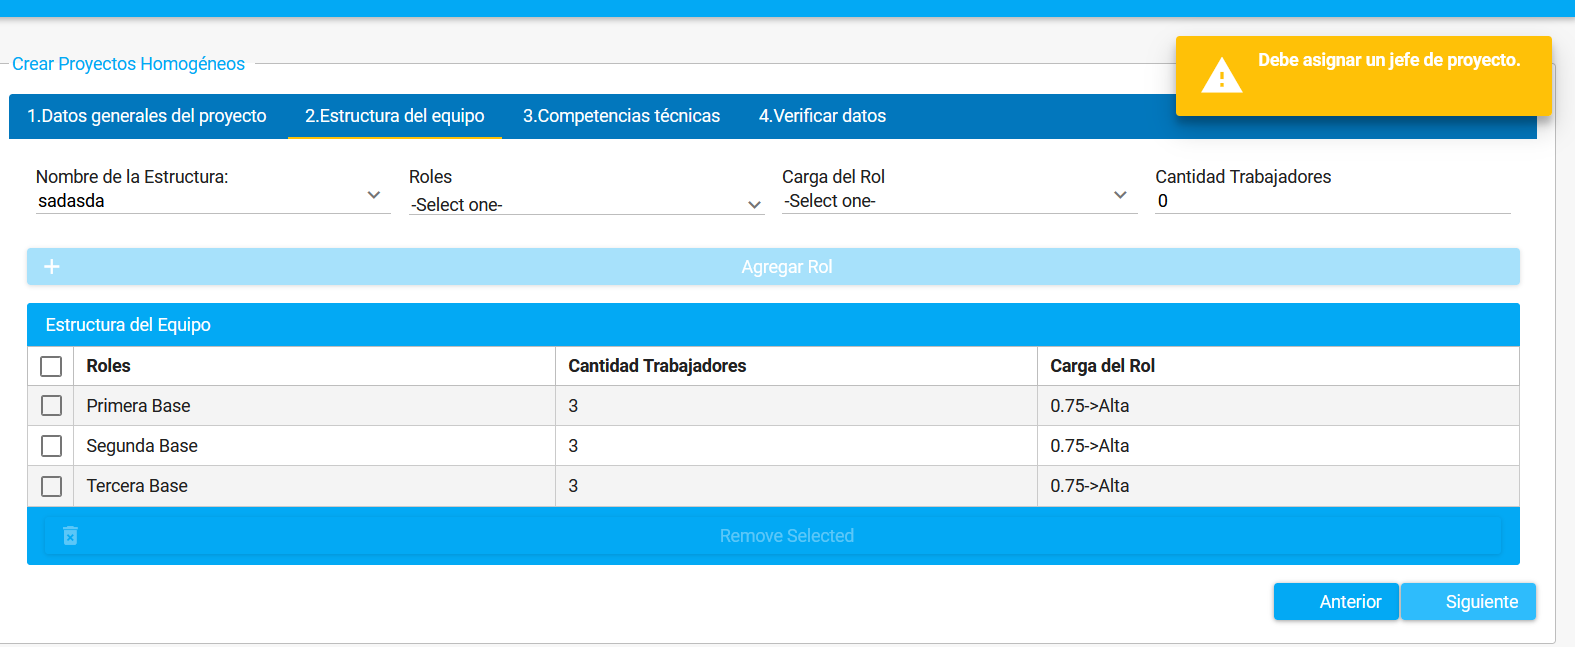
\includegraphics[width=0.9\textwidth]{figuras/error-jefe-proy.png}
	\caption{Error al crear estructura sin Jefe de Proyecto} \label{fig:error-jefe-proy}
\end{figure}

Confirmando los CP realizados, la Figura \ref{fig:apariciones-jefe-proy} muestra alguna de las apariciones de la cadena \textit{Jefe de Proyecto} en el código fuente de la herramienta.

\begin{figure}[H]
	\centering
	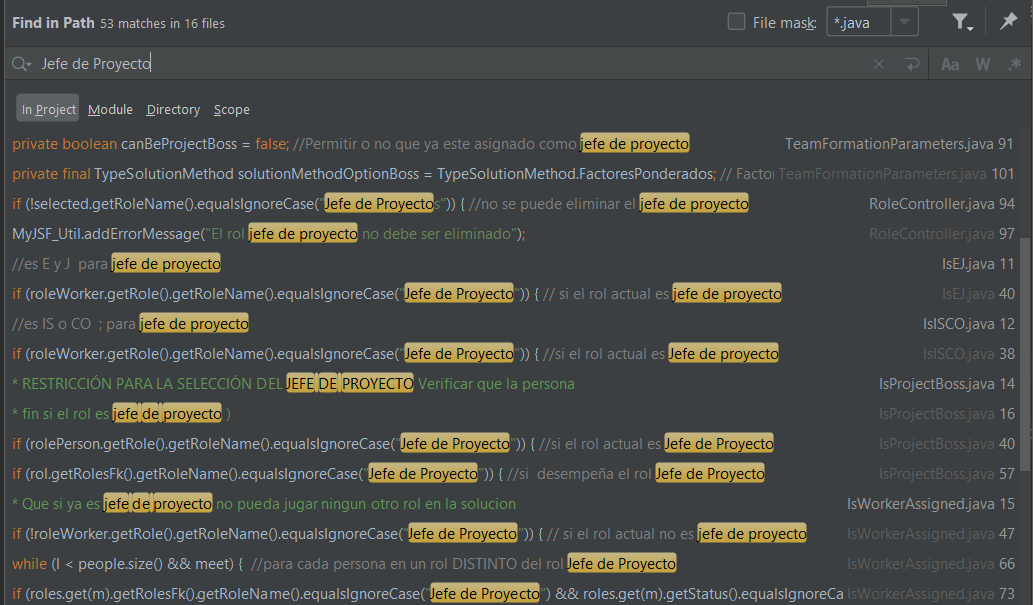
\includegraphics[width=\textwidth]{figuras/string-texto-jefe-proy.png}
	\caption{Apariciones del texto \textit{Jefe de Proyecto}} \label{fig:apariciones-jefe-proy}
\end{figure}

Específicamente, a la hora de validar una estructura, se verifica que en esta exista un rol con el nombre: \textit{Jefe de Proyecto}. La Figura \ref{fig:cod-valida} muestra lo planteado.

\begin{figure}[H]
	\centering
	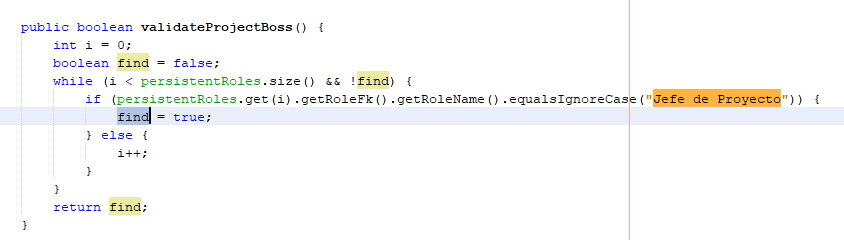
\includegraphics[width=\textwidth]{figuras/validate-state.png}
	\caption{Código utilizado para validar la presencia del rol Jefe de Proyecto} \label{fig:cod-valida}
\end{figure}

%Otro aspecto a resaltar es la entrada de datos. En el sistema, este proceso solo se puede realizar de forma manual. Y cuando existen muchas personas a incorporar, se puede considerar como un proceso largo y tedioso. En adición, el sistema no se encuentra preparado para especificar que se va a trabajar con un tipo de problema en particular. Entonces, las ecuaciones propuestas para el cálculo de las competencias $t_4$ (\ref{ec:embase}) y $t_5$ (\ref{ec:pos}) correspondientes al problema del béisbol, no se podrán modelar en el sistema, debido a que no son lo suficientemente generales para extenderlas . \\

Las personas tienen generalmente cierta experiencia trabajando. Por ejemplo, un recién graduado tiene menos experiencia como profesional que una persona que lleva trabajando 10 años en la industria. Esta última, se ha enfrentado a múltiples problemas, y debe saber cómo solucionarlos debido a su experiencia. Este atributo no se encuentra modelado actualmente en TEAMSOFT$^+$. \\ 

La internacionalización de un sitio web consiste en identificar toda la información cambiante en función del idioma de preferencia del usuario. TEAMSOFT$^+$ tiene presente esta característica. Sin embargo, no está funcional. Esto no afecta al proceso de formación de equipos, pero sigue siendo una limitación.

\section{Generación de soluciones en los problemas de docencia y béisbol}
En esta sección se realizan los experimentos asociados a ambos problemas con los datos de la importación de las personas mencionados en las secciones \ref{sec:impo_docencia} y \ref{sec:impo_beisbol}. Para comprobar la efectividad de las soluciones propuestas con TEAMSOFT$^+$ a ambos modelos se realizan un conjunto de experimentos teniendo en cuenta las características propias de cada problema, el uso de diferentes FO y algoritmos de solución. Para ambos problemas se utilizaron los siguientes algoritmos disponibles en la herramienta: 
\begin{itemize}
%	\setlength\itemsep{0em}
	\item Escalador de colinas (EC)
	\item Escalador de colinas con reinicio (ECR)
	\item Búsqueda aleatoria (BA)
\end{itemize}

Se realizaron 20 ejecuciones por cada algoritmo y 3000 iteraciones. En el caso del algoritmo ECR, se establece 100 como máximo número de iteraciones para que el algoritmo se reinicie. Para definir el valor de cumplimiento de las competencias, se definen cuatro niveles. En la Tabla \ref{table:niveles} se muestra cada nivel definido y su significado. Mientras más grande sea el valor del nivel mayor es su significado.

\begin{table}[H]
	\centering
	\caption{Niveles definidos para el cumplimiento de las competencias}\label{table:niveles}
%	\scalebox{.95}{
	\begin{tabular}{c l}
		\toprule
		\textbf{Nivel} & \textbf{Significado} \\ \midrule
		1              & En partida           \\
		2              & En desarrollo        \\
		3              & En avance            \\
		4              & Experto              \\ \bottomrule
	\end{tabular}
%	}
\end{table}

\subsection{Solución al problema de docencia}
El problema de la docencia tiene algunos aspectos particulares: 
\begin{itemize}
%	\setlength\itemsep{0em}
	\item No existen incompatibilidades definidas entre los roles.
	\item Los profesores pueden estar asignados a más de una asignatura, siempre y cuando la carga de trabajo no sobrepase el valor límite.
	\item En ocasiones, se necesita que la persona que desempeña el rol Líder ocupe otro rol dentro de la misma asignatura.
\end{itemize}

Es importante volver a recalcar que en este problema, las asignaturas a impartir, se consideran como equipos a formar. Además, a decisión del autor, se decide utilizar los datos de los profesores asociados a la disciplina Inteligencia Computacional. La Tabla \ref{table:nivel-pers-comp} refleja los niveles de los profesores en cada competencia, calculados a partir de la importación. Solo se presentan los primeros cinco, el resto puede ser consultado en el Anexo \ref{table:nivel-pers-comp2}.\\

\vspace{-1cm}
\begin{table}[H]
	\centering
	%	\hspace{-4cm}
	\caption{Nivel de los profesores por competencias: Trabajo docente (TD), Trabajo metodológico (TM), Trabajo investigativo (TI), Categoría docente (CD) y Grado científico (GC)}\label{table:nivel-pers-comp}
	\scalebox{.9}{
		\begin{tabular}{l l l l l l }
			\toprule
			\multirow{2}{2.5cm}{\textbf{Profesor}} &                  \multicolumn{5}{c}{\textbf{Competencias}}                  \\ \cline{2-6}
			                                       & \textbf{TD}   & \textbf{TM}   & \textbf{TI}   & \textbf{CD} & \textbf{GC}   \\ \midrule
			Raisa Socorro                          & Experto       & Experto       & En desarrollo & Experto     & Experto       \\ \hline
			Alejandro Rosete                       & Experto       & Experto       & Experto       & Experto     & Experto       \\ \hline
			Maylin                                 & Experto       & Experto       & Experto       & Experto     & Experto       \\ \hline
			Luis                                   & En desarrollo & En desarrollo & En desarrollo & En partida  & En desarrollo \\ \hline
			Camila                                 & En desarrollo & En desarrollo & En desarrollo & En partida  & En desarrollo \\ \hline
			...                                    & ...           & ...           & ...           & ...         & ...           \\ \bottomrule
		\end{tabular}
	}
\end{table}

También calculado a partir de los datos del fichero, se obtiene la experiencia de las personas por los roles.  La Tabla \ref{table:pref-pers-roles-doc} refleja con una $X$ la preferencia de la persona $p_i$ por el rol $r_i$. Se deben formar los equipos de profesores para impartir las asignaturas Matemática Discreta (MD), Inteligencia Artificial (IA) y Metodología de la Investigación (MI). Se escogen estas asignaturas debido a que todas se imparten en el mismo semestre.  Para configurar un equipo es necesario primero definir los roles que se deben cubrir, la cantidad de personas que se necesitan para desempeñar cada rol y, la carga que le conlleva al trabajador desempeñar cada rol. Las Tabla \ref{table:asig_rol} muestra las configuraciones establecidas para cada una de las asignaturas seleccionadas.


\begin{table}[H]
	\centering
	%	\hspace{-2cm}
	\caption{Preferencia de las personas por los roles: Líder (L), Conferencia (C), Clase práctica (CP), Seminario (S), Laboratorio (LB) y Taller (T)}\label{table:pref-pers-roles-doc}
%		\scalebox{.87}{
	\begin{tabular}{l c c c c c c }
		\toprule
		\multirow{2}{2.5cm}{\textbf{Profesor}} &                                              \multicolumn{6}{c}{\textbf{Roles}}                                               \\ \cline{2-7}
		& \textbf{L} & \textbf{C} & \textbf{CP} & \textbf{S} & \textbf{LB} & \textbf{T} \\ \midrule
		Raisa Socorro                          & X              & X                    & X                       &                    &  \\ \hline
		Alejandro Rosete                       & X              & X                    & X                       & X                  &  \\ \hline
		Maylin                                 & X              & X                    & X                       & X                  &  \\ \hline
		Luis                                   &                &                      &                         &                    &  \\ \hline
		Camila                                 &                &                      &                         &                    &  \\ \hline
		...                                    & ...            & ...                  & ...                     & ...                & ...                  & ...             \\ \bottomrule
	\end{tabular}
%	}
\end{table}


%-----------------------------------empiezan los proyectos-------------------

%Las asignaturas Matemática Discreta (MD), Inteligencia Artificial (IA) y Metodología de la Investigación (MI) serán los proyectos a solucionar. Se escogen estas asignaturas debido a que todas se imparten en el mismo semestre.  Para configurar un proyecto es necesario primero definir los roles que lo conforman, la cantidad de personas que se necesitan para desempeñar cada rol y, la carga que le conlleva al trabajador desempeñarlo. Las Tabla \ref{table:asig_rol} muestra las configuraciones establecidas para cada una de las asignaturas seleccionadas. 

\begin{table}[H]
	\centering
%	\hspace{-2cm}
	\caption{Configuración de los roles para cada una de las asignaturas} \label{table:asig_rol}
		\scalebox{.95}{
	\begin{tabular}{ | l | c | c | c | c | c | c |}
		\toprule
		\multirow{3}{3cm}{\textbf{Rol}} &                                         \multicolumn{6}{c|}{\textbf{Asignatura}}                                         \\
		\cmidrule{2-7}                  &    \multicolumn{2}{c|}{\textbf{MD}}    &    \multicolumn{2}{c|}{\textbf{IA}}    &    \multicolumn{2}{c|}{\textbf{MI}}    \\
		\cmidrule{2-7}                  & \textbf{No. personas} & \textbf{Carga} & \textbf{No. personas} & \textbf{Carga} & \textbf{No. personas} & \textbf{Carga} \\ \midrule
		Líder                           & 1                     & media          & 1                     & media          & 1                     & media          \\ \hline
		Conferencia                     & 1                     & media          & 1                     & media          & 1                     & baja           \\ \hline
		Seminario                       & 3                     & baja           & --                    & --             & 1                     & baja           \\ \hline
		Clase Práctica                  & --                    & --             & 2                     & media          & --                    & --             \\ \bottomrule
	\end{tabular}
	}
\end{table}

%----------------------------terminan los proyectos-----------------------------------

Una vez establecidos los roles, la cantidad de personas y la carga para cada rol, es necesario definir las competencias necesarias para que una persona pueda desempeñar cada rol. En este caso, para cada asignatura se decidió establecer a los roles de Líder y Conferencia, todas las competencias con el máximo nivel: Experto. Un ejemplo de esta configuración se puede consultar en el Anexo \ref{fig:conf-roles-comp-asignatura}. \\ 

TEAMSOFT$^+$ permite diferentes configuraciones a tener en cuenta para formar los equipos. Las soluciones que se presentan en esta sección se obtienen utilizando múltiples equipos (tres asignaturas), con el método de que conforma los equipos de forma simultánea, asignando primero a los jefe de asignaturas (Líder). Se utiliza la nueva restricción  incorporada a la herramienta, la cual establece que el Líder del proyecto tiene que desempeñar otro rol dentro del mismo equipo (el jefe de asignatura tiene que impartir esta asignatura). \\

%\subsubsection{Solución al problema}

Para resolver el problema se utiliza una función multiobjetivo que tiene en cuenta los siguientes criterios:
\begin{enumerate}
	\setlength\itemsep{0em}
	\item Maximizar competencias (C)
	\item Balancear la carga de trabajo entre equipos (BCT)
	\item Maximizar intereses de las personas por los roles (P)
\end{enumerate}

En relación con la función objetivo BTC, se establece 1.0 como límite de carga máxima que puede tener un profesor. La solución inicial se construye utilizando el método propuesto en el Capítulo \ref{chap:2} que garantiza una solución inicial que cumpla la restricción de que el jefe de asignatura imparta la asignatura en cualquiera de sus roles. Además, se emplea un operador de mutación que sustituye a un profesor en una asignatura por otro cualquiera, en todos los roles que desempeña en esa asignatura. En la Tabla \ref{table:resultados-docencia} se muestran los resultados obtenidos después de diez corridas utilizando los algoritmos disponibles en TEAMSOFT$^+$. La mejor solución se señala en gris. Como se puede observar, la mejor solución teniendo en cuenta las tres FO se obtiene a partir de la aplicación del algoritmo EC.

\begin{table}[H]
	\centering
	\caption{Resultado de la evaluación de los algoritmos: Escalador de colinas (EC), Escalador de colinas con reinicio (ECR), Búsqueda aleatoria (BA) y Búsqueda Tabú (BT) en las FO} \label{table:resultados-docencia}
\scalebox{.9}{
	\begin{tabular}{|c | c | c| c | c |c |c | c| c| c |}
		\toprule
		\multirow{3}{1cm}{\textbf{No.}} &                       \multicolumn{3}{c|}{\textbf{EC}}                        &   \multicolumn{3}{c|}{\textbf{ECR}}    &    \multicolumn{3}{c|}{\textbf{BA}}      \\
		        \cmidrule{2-10}         & \textbf{C}               & \textbf{P}               & \textbf{BCT}            & \textbf{C} & \textbf{P} & \textbf{BCT} & \textbf{C} & \textbf{P} & \textbf{BCT}   \\ \midrule
		               1                & 0.97                     & 0.83                     & 1.00                    & 0.97       & 0.83       & 1.00         & 0.97       & 0.83       & 0.62           \\ \hline
		               2                & 0.98                     & 0.83                     & 0.83                    & 0.98       & 0.91       & 1.00         & 0.96       & 0.83       & 0.58           \\ \hline
		               3                & 0.95                     & 1.00                     & 1.00                    & 0.97       & 0.91       & 1.00         & 0.97       & 0.83       & 0.79           \\ \hline
		               4                & 0.96                     & 1.00                     & 1.00                    & 0.96       & 1.00       & 1.00         & 0.95       & 0.91       & 1.00           \\ \hline
		               5                & \cellcolor{gray!30} 0.97 & \cellcolor{gray!30} 1.00 & \cellcolor{gray!30}1.00 & 0.97       & 0.75       & 1.00         & 0.96       & 0.91       & 1.00           \\ \hline
		               6                & 0.98                     & 0.91                     & 1.00                    & 0.95       & 1.00       & 1.00         & 0.96       & 0.75       & 1.00           \\ \hline
		               7                & 0.95                     & 0.83                     & 1.00                    & 0.98       & 0.83       & 0.83         & 0.97       & 0.83       & 0.79           \\ \hline
		               8                & 0.97                     & 0.93                     & 1.00                    & 0.98       & 0.75       & 0.83         & 0.95       & 1.00       & 1.00           \\ \hline
		               9                & 0.96                     & 1.00                     & 1.00                    & 0.95       & 0.75       & 1.00         & 0.98       & 0.83       & 1.00           \\ \hline
		              10                & 0.97                     & 0.91                     & 0.8333                  & 0.97       & 0.91       & 1.00         & 0.98       & 0.83       & 1.00           \\ \bottomrule
	\end{tabular}
}
\end{table}

La Tabla \ref{table:asingnacion-doc} muestra los resultados de la mejor solución encontrada al realizar el proceso de asignación de los profesores a los roles en las asignaturas. En el Anexo \ref{fig:solucion-docencia} se muestra una captura de pantalla de esta solución desde la herramienta.

\begin{table}[H]
	\centering
	\caption{Asignación con mejor puntuación por el algoritmo EC} \label{table:asingnacion-doc}
	\begin{tabular}{l p{3.3cm} l l}
		\toprule
		\textbf{Rol}                      & \textbf{MD}           & \textbf{IA}           & \textbf{MI}               \\ \midrule
		Líder                             & Alejandro Rosete      & Maylin                & Raisa Socorro                    \\ \hline
		Conferencia                       & Maylin                & Maylin                & Raisa Socorro         \\ \hline
		\multirow{2}{3cm}{Clase Práctica} & \multirow{2}{2cm}{--} & Milton               & \multirow{2}{2cm}{--}     \\
		                                  &                       & Raisa Socorro                 &  \\ \hline
		\multirow{3}{2cm}{Seminario}      & Alejandro Rosete      & \multirow{3}{2cm}{--} & \multirow{3}{2cm}{Alfredo} \\
		                                  & Alfredo               &                       &  \\
		                                  & Ernesto               &                       &  \\ \bottomrule
	\end{tabular}
\end{table}
 
La Tabla \ref{table:asignacion-jefe-departamento} muestra la asignación de los profesores a las asignaturas realizada por el jefe de departamento.

 \begin{table}[H]
 	\centering
 	\caption{Asignación realizada por el jefe de departamento} \label{table:asignacion-jefe-departamento}
 	\begin{tabular}{l p{3.3cm} l l}
 		\toprule
 		\textbf{Rol}                      & \textbf{MD}           & \textbf{IA}           & \textbf{MI}              \\ \midrule
 		Líder                             & Alejandro Rosete      & Maylin                & Maylin                   \\ \hline
 		Conferencia                       & Alejandro Rosete      & Maylin                & Maylin                   \\ \hline
 		\multirow{2}{3cm}{Clase Práctica} & \multirow{2}{2cm}{--} & Eduardo               & \multirow{2}{2cm}{--}    \\
 		                                  &                       & Anabel                &  \\ \hline
 		\multirow{3}{2cm}{Seminario}      & Wenny                 & \multirow{3}{2cm}{--} & \multirow{3}{2cm}{Vilma} \\
 		                                  & David                 &                       &  \\
 		                                  & Alejandro Rosete      &                       &  \\ \bottomrule
 	\end{tabular}
 \end{table}
  
En ambas soluciones se cumplen los niveles mínimos requeridos en las competencias para desempeñar  los roles. También se cumple que el Líder tiene que formar parte del claustro de profesores de la asignatura. Por último, la carga docente en cada caso no excede el límite. Aunque si se desea evitar que el profesor esté muy cargado, este valor es configurable. Es importante resaltar que en el caso de la solución realizada por el jefe de departamento, se tienen en cuenta las preferencias de las personas por las asignaturas, lo cual no se tuvo en cuenta en la solución propuesta en los algoritmos debido a que está en proceso de implementación por otro equipo de desarrollo.
 
\subsection{Solución al problema de  béisbol}

El contexto de formación de un equipo de béisbol, tiene características que se diferencia tanto del problema formación de equipos de profesores para impartir docencia, como en la formación de equipos de proyectos de software. Estas particularidades consisten en: 
\begin{itemize}
	\setlength\itemsep{0em}
	\item 144 incompatibilidades entre los roles a desempeñar por los jugadores.
	\item Los jugadores tienen que ocupar como mínimo dos roles.
	\item Los jugadores pueden ocupar como máximo tres roles.
\end{itemize}

Además, a decisión del autor, se decide utilizar como ejemplo los datos de los jugadores del equipo de Matanzas de la Serie Nacional. La Tabla \ref{table:nivel-jugadores-comp} refleja los niveles de los jugadores en cada competencia, calculados a partir de la importación. Solo se presentan los primeros cinco, el resto puede ser consultado en el Anexo \ref{table:nivel-jugadores-comp2}.

\begin{table}[H]
	\centering
	%	\hspace{-4cm}
	\caption{Nivel de los jugadores en las competencias: Batear con hombres en base (B), Fuerza de bateo (F), Precisión de tiro (P), Capacidad de embase (E) y Velocidad (V)}\label{table:nivel-jugadores-comp}
	\scalebox{.95}{
		\begin{tabular}{l l l l l l }
			\toprule
			\multirow{2}{2.5cm}{\textbf{Jugador}} &                 \multicolumn{5}{c}{\textbf{Competencias}}                  \\ \cline{2-6}
			                                      & \textbf{B}    & \textbf{F}    & \textbf{P} & \textbf{E}    & \textbf{V}    \\ \midrule
			Yurisbel Gracial                      & En partida    & En desarrollo & Experto    & En desarrollo & En partida    \\ \hline
			Jefferson Delgado                     & En avance     & En desarrollo & Experto    & En avance     & En desarrollo \\ \hline
			Ariel Sánchez                         & En avance     & En desarrollo & Experto    & En avance     & En partida    \\ \hline
			Yasiel Santoya                        & En desarrollo & En desarrollo & Experto    & En desarrollo & En partida    \\ \hline
			Andrys Pérez                          & En desarrollo & En partida    & Experto    & En desarrollo & En partida    \\ \hline
			...                                   & ...           & ...           & ...        & ...           & ...           \\ \bottomrule
		\end{tabular}
	}
\end{table}

En la Tabla \ref{table:pref-pers-roles-pel} se muestran las preferencias de los jugadores por los roles. Estos datos son el resultado de la importación del fichero de entrada. Como se puede observar, los jugadores solo tienen algunos roles asociados. La ausencia de un rol significa que no es de su preferencia. Teniendo en cuenta el número de jugadores del equipo solo se muestran los cinco primeros, el resto puede ser consultado en el Anexo \ref{table:pref-pers-roles-pel2}.

\begin{table}[H]
	\centering
	%	\hspace{-4cm}
	\caption{Preferencia de los jugadores por los roles}\label{table:pref-pers-roles-pel}
%	\scalebox{.95}{
		\begin{tabular}{l l }
			\toprule
			\textbf{Jugador}  & \textbf{Roles}             \\ \midrule
			Yurisbel Gracial  & B3, B4, 3B        \\ \hline
			Jefferson Delgado & 3B                \\ \hline
			Ariel Sánchez     & B3, LF            \\ \hline
			Yasiel Santoya    & B3, B4, 1B, Líder \\ \hline
			Andrys Pérez      & B8, B9, C         \\ \hline
			...               & ...               \\ \bottomrule
		\end{tabular}
%	}
\end{table}

En el béisbol, en algunas posiciones resulta más importantes tener en cuenta, durante el proceso de asignación, las competencias de los jugadores para ocupar estas posiciones. Para modelar esta situación TEAMSOFT$^+$ define la importancia de los roles en un equipo. Utilizando esta funcionalidad, se definen para el béisbol nueve niveles de importancia, donde un mayor nivel implica mayor importancia. Entre los roles defensivos, el Receptor, el Campo corto y el Jardín central cumplen una función defensiva muy importante, es por esto que se les asigna los mayores niveles de importancia. Los primeros cinco roles a la ofensiva también juegan un gran papel en el equipo. A ellos les corresponde entonces altos niveles de importancia. En el Anexo \ref{fig:conf-roles-comp-pelota1} se presenta los niveles utilizados para cada uno de los roles. Estos niveles pueden ser configurados a criterio del especialista a cargo de la selección del equipo.	\\

Para configurar un equipo es necesario primero definir los roles que lo conforman, la cantidad de personas que se necesitan para desempeñar cada rol y, la carga que implica al jugador su desempeño. Los roles asociados a este problema fueron definidos en el Capítulo \ref{chap:2}, así como la cantidad de jugadores necesarios para desempeñar cada uno. La carga de trabajo asociada a un rol no es relevante, debido a que solo se va a formar un equipo. Una vez establecidos los roles y la cantidad de jugadores por rol, es necesario definir las competencias necesarias para que un jugador pueda desempeñar cada rol. Todas estas configuraciones se pueden consultar en los Anexos \ref{fig:conf-equipo-pelota1}, \ref{fig:conf-equipo-pelota2}, \ref{fig:conf-equipo-pelota3}, \ref{fig:conf-equipo-pelota4}. \\

TEAMSOFT$^+$ permite diferentes configuraciones a tener en cuenta para formar los equipos. Las soluciones que se presentan en esta sección se obtienen utilizando un solo equipo, con el método: Formar equipos de uno en uno, con la variante de no asignar primero al Líder. Se utiliza una nueva restricción  incorporada a la herramienta, la cual establece que todos los miembros del equipo tienen que ocupar todos al menos $n$ roles, siendo en este caso $n=2$, ocupando un rol a la ofensiva y otro a la defensiva. Esto último se garantiza por las incompatibilidades establecidas entre los roles. Además, se establece tres roles como cantidad máxima a ocupar por una persona. Esto se debe a que el Líder además de ocupar su rol, puede ocupar también un rol a la defensiva y uno a la ofensiva.\\

%\subsubsection{Solución al problema}

Las funciones objetivos seleccionadas fueron:
\begin{enumerate}
	\setlength\itemsep{0em}
	\item Maximizar competencias (C)
	\item Maximizar preferencias de las personas por los roles (P)
\end{enumerate}

Además, se establece la restricción de que no pueden existir incompatibilidades entre los roles ocupados por los jugadores. La solución inicial se construye utilizando el método propuesto en el Capítulo \ref{chap:2} que garantiza una solución inicial que cumpla la restricción de que una persona tiene que estar asignada como mínimo a dos roles. Se emplea un operador de mutación que sustituye a un jugador por otro cualquiera en todos los roles que desempeña en el equipo. \\

En la Tabla \ref{table:resultados-beisbol} se muestran los resultados obtenidos después de diez corridas utilizando los algoritmos disponibles en TEAMSOFT$^+$. La mejor solución se señala en gris. Puede consultar para más detalles el Anexo \ref{fig:solucion-beisbol}. Como se puede observar, la mejor solución teniendo en cuenta las tres FO se obtiene a partir de la aplicación del algoritmo Escalador de Colinas con Reinicio. \\

Las Tablas \ref{table:asignacion-pelota-def} y \ref{table:asignacion-pelota-of} muestran las asignaciones realizadas por el \textit{Manager} (tomado del sitio web beisbolcubano \cite{SN21}) y la mejor solución encontrada para los roles defensivos y ofensivos respectivamente. Las propuestas coincidentes son resaltadas en gris. Se puede observar que existen cinco coincidencias en total, dos de ellas en la alineación defensiva, y tres en la alineación ofensiva. A pesar de esto, los jugadores asignados cumplen las competencias, definidas en la configuración utilizada, para desempeñar el rol asignado. Entre las no coincidencias se encuentra, la asignación realizada al jugador Yurisbel Gracial, este se encontraba en esos momentos contratado en la liga japonesa de béisbol en el equipo \textit{Halcones de Softbank}, y además de cumplir las competencias para los roles asignados, históricamente ha jugado estas posiciones. Para el caso de Yasiel Santoya, ha sido polémica su ausencia en la alineación del equipo de Matanzas. A lo largo de su carrera ha desempeñado el rol de antesalista (1B) y ha alternado entre los puestos B3, B4, B5 tanto en el equipo de Sancti Spíritus, como en el propio Matanzas. \\

A pesar de lo antes mencionado, la asignación de los jugadores realizada por el algoritmo que no coinciden con la alineación del \textit{manager} pueden jugar ese rol sin ningún problema debido a que poseen las competencias para hacerlo. Este es el caso de Brian Rodríguez, joven promesa del equipo matancero, que en su debut en esta serie ha jugado como B4 y 1B. Por sus pocas apariciones al bate y buenos resultados presenta un \textbf{OBP} y un \textbf{AVE} ofensivo que lo califican para ocupar el rol BD y B2. En el caso de Yariel Duque, a pesar que el \textit{manager} lo asigna como 1B, en este caso esa posición ha sido asignada a Yasiel Santoya, quien cumple también con las competencias e históricamente, ocupante de esa posición. Yariel Duque entonces es asignado como LF, posición para la cual tiene condiciones \cite{RofesPerez2016}. Un caso curioso es el de Erisbel Arruebarruena, en la alineación del \textit{manager} mostrada no coincide como B7, sin embargo en las restantes alineaciones de la final, sí ocupó este orden al bate. Todos los jugadores cumplen con las competencias configuradas para los roles que fueron asignados. Los niveles de los jugadores en las competencias se pueden consultar en el Anexo \ref{table:nivel-jugadores-comp2} y los niveles necesarios para ocupar una posición se pueden consultar en el Anexo \ref{fig:conf-roles-comp-asignatura}.


\begin{table}[H]
	\centering
	\caption{Resultado de la evaluación de los algoritmos: Escalador de colinas (EC), Escalador de colinas con reinicio (ECR) y Búsqueda aleatoria (BA) en las FO} \label{table:resultados-beisbol}
%	\scalebox{.9}{
	\begin{tabular}{| c | c | c| c | c | c | c |}
		\toprule
		\multirow{2}{1cm}{\textbf{No.}} & \multicolumn{2}{c|}{\textbf{EC}} &         \multicolumn{2}{c|}{\textbf{ECR}}         & \multicolumn{2}{c|}{\textbf{BA}} \\ \cmidrule{2-7} 
		& \textbf{C} & \textbf{P} & \textbf{C} & \textbf{P} & \textbf{C} & \textbf{P} \\ \midrule
		1                               & 0.56 & 0.31                      & 0.57                    & 0.42                    & 0.6  & 0.47         \\ \hline
		2                               & 0.55 & 0.47                      & 0.56                    & 0.57                    & 0.55 & 0.21         \\ \hline
		3                               & 0.6  & 0.31                      & 0.55                    & 0.42                    & 0.58 & 0.21         \\ \hline
		4                               & 0.54 & 0.57                      & 0.55                    & 0.57                    & 0.59 & 0.21         \\ \hline
		5                               & 0.48 & 0.63                      & 0.6                     & 0.26                    & 0.56 & 0.36         \\ \hline
		6                               & 0.59 & 0.52                      & 0.56                    & 0.31                    & 0.53 & 0.52         \\ \hline
		7                               & 0.59 & 0.41                      & 0.54                    & 0.57                    & 0.58 & 0.21         \\ \hline
		8                               & 0.53 & 0.57                      & 0.58                    & 0.42                    & 0.53 & 0.52         \\ \hline
		9                               & 0.56 & 0.52                      & 0.58                    & 0.31                    & 0.55 & 0.1          \\ \hline
		10                              & 0.57 & 0.52                      & \cellcolor{gray!30} 0.56 & \cellcolor{gray!30}0.68 & 0.57 & 0.26         \\ \bottomrule
	\end{tabular}
%}
\end{table}


\begin{table}[H]
	\centering
	\caption{Resultado de la asignación de la mejor solución encontrada para los roles defensivos}\label{table:asignacion-pelota-def}
%		\scalebox{0.95}{
	\begin{tabular}{l l l }
		\toprule
		\textbf{Rol}         & \textbf{Alineación del \textit{Manager}} & \textbf{Alineación del algoritmo} \\ \midrule
		\rowcolor{gray!30} C & Andrys Pérez                             & Andrys Pérez                      \\
		1B                   & Yariel Duque                             & Yasiel Santoya                    \\
		\rowcolor{gray!30}2B & Aníbal Medina                            & Aníbal Medina                     \\
		\rowcolor{gray!30}SS & Erisbel Arruebaruena                     & Erisbel Arruebaruena              \\
		3B                   & Yadil Mujica                             & Yurisbel Gracial                  \\
		LF                   & Ariel Sánchez                            & Yariel Duque                      \\
		CF                   & Eduardo Blanco                           & Yadil Mujica                      \\
		\rowcolor{gray!30}RF & Willian Luis                             & Willian Luis                      \\
		BD                   & Jefferson Delgado                        & Brian Rodríguez                   \\ \bottomrule
	\end{tabular}
%		}
\end{table}

\begin{table}[H]
	\centering
	\caption{Resultados de la asignación de la mejor solución encontrada para los roles ofensivos y la alineación realizada por el \textit{manager} en la final con mayor coincidencia}\label{table:asignacion-pelota-of}
	%	\scalebox{0.95}{
	\begin{tabular}{l l l }
		\toprule
		\textbf{Rol}          & \textbf{Alineación del \textit{manager}} & \textbf{Alineación del algoritmo} \\ \midrule
		B1                    & Aníbal Medina                            & Yadil Mujica                      \\
		B2                    & Yadil Mujica                             & Brian Rodríguez                   \\
		B3                    & Ariel Sánchez                            & Yurisbel Gracial                  \\
		B4                    & Erisbel Arruebaruena                     & Yasiel Santoya                    \\
		B5                    & Yariel Duque                             & Willian Luis                      \\
		B6  & Jefferson Delgado                        & Yariel Duque                      \\
			B7 & Willian Luis                             & Erisbel Arruebaruena              \\
		\rowcolor{gray!30}	B8 & Andrys Pérez                             & Andrys Pérez                      \\
		B9                    & Eduardo Blanco                           & Aníbal Medina                     \\ \bottomrule
	\end{tabular}
	%	}
\end{table}
%
%A pesar de lo antes mencionado, la asignación de los jugadores realizada por el algoritmo que no coinciden con la alineación del \textit{manager} pueden jugar ese rol sin ningún problema debido a que poseen las competencias para hacerlo.

\section{Conclusiones}
Con la culminación de este capítulo, se arribaron a las siguientes conclusiones:
\begin{enumerate}
	\item Se verifica que el proceso de importación de los datos se realice de manera correcta, en tanto, se logran importar los datos para formar equipo en ambos contextos analizados.
	\item Tanto las competencias como los indicadores empleados para determinar el cumplimiento de las mismas, deben ser refinadas por un experto en cada tema, de modo que se refleje mejor los aspectos a tener en cuenta al formar estos equipos. La herramienta permite establecer esta configuración.
	\item Se lograron obtener propuestas de equipos utilizando la herramienta TEAMSOFT$^+$ en ambos contextos (béisbol y profesores para impartir docencia).
	\item Las propuestas obtenidas para los equipos docentes cumplen con todas las restricciones establecidas que exige el problema. Sin embargo, los equipos difieren de los formados por el jefe de departamento (de forma manual) ya que no se modeló el factor de preferencia de los profesores por las asignaturas.
	\item A pesar del gran número de restricciones y roles a cubrir presentes en la formación de equipos de béisbol, se generaron soluciones factibles. Aunque no hubo coincidencia total con las alineaciones registradas por el \textit{manager} del equipo, todos los asignados cumplen con las competencias para ocupar estas posiciones, y algunos se han desempeñado en estas posiciones con anterioridad.
\end{enumerate}

